\documentclass{article}

% NeurIPS 2024 style
\usepackage[final]{neurips_2024}

\usepackage[utf8]{inputenc}
\usepackage[T1]{fontenc}
\usepackage[french]{babel}
\usepackage{hyperref}
\usepackage{url}
\usepackage{booktabs}
\usepackage{amsfonts}
\usepackage{nicefrac}
\usepackage{microtype}
\usepackage{xcolor}
\usepackage{graphicx}
\usepackage{subfigure}
\usepackage{multirow}
\usepackage{array}
\usepackage{natbib}

% ── Métadonnées ───────────────────────────────────────────────────────────────
\title{Cadrage partisan et variations stylistiques dans les professions de foi :\\
une analyse computationnelle du corpus Archelec 1993}

\author{%
  Dominique Noutsougankom\\
  ENSAE Paris\\
  \texttt{noutsougankomladominique@gmail.com}
}

% ─────────────────────────────────────────────────────────────────────────────
\begin{document}
\maketitle

% ── Résumé ───────────────────────────────────────────────────────────────────
\begin{abstract}
Ce travail propose une analyse computationnelle du corpus Archelec des élections
législatives françaises de 1993 (5\,835 professions de foi).
Nous poursuivons deux objectifs complémentaires.
Le premier est de cartographier les structures thématiques du discours électoral
à l'aide de trois méthodes de modélisation thématique : LDA, NMF et BERTopic.
La LDA avec $K=10$ thèmes (cohérence $C_v = 0.654$) révèle une spécialisation
partisane forte : le Front national est concentré sur le thème immigration
(indice $\times 8.35$), l'extrême gauche sur la lutte des classes ($\times 13.45$),
tandis que le clivage au sein de l'écologie (Verts vs. CPNT) émerge nettement
avec la NMF. BERTopic, en revanche, produit un cluster dominant regroupant
72\,\% des documents, ce qui révèle une homogénéité sémantique de surface
qui limite sa discrimination sur ce corpus particulier.
Le second objectif est d'examiner si le sexe des candidats est associé à
des patterns stylistiques mesurables.
Sur 20 features extraites de la littérature en stylométrie computationnelle,
9 sont robustes à la fois aux tests de Mann-Whitney (correction de Bonferroni)
et aux régressions OLS avec contrôle du parti.
Le signal de genre réside principalement dans la structure syntaxique et
non dans le vocabulaire~: les femmes candidates emploient davantage de
déterminants, de nominalisations et de formulations de doute, tandis que
les hommes referencent plus fréquemment des noms propres par voie prépositionnelle.
\end{abstract}

% ── 1. Introduction ───────────────────────────────────────────────────────────
\section{Introduction}
\label{sec:intro}

Les professions de foi occupent une place singulière dans le système électoral
français. Distribuées à l'ensemble des électeurs d'une circonscription par
les services de l'État, elles constituent l'un des rares supports où chaque
candidat~--- des grandes formations aux mouvements marginaux~--- dispose d'un
espace identique pour formuler son programme et convaincre ses concitoyens.
À ce titre, elles forment un corpus d'une remarquable cohérence formelle :
même contrainte de mise en page, même moment de rédaction, même audience cible.
Cette homogénéité en fait un matériau particulièrement adapté aux méthodes
quantitatives d'analyse textuelle.

L'approche \emph{Text as Data} \citep{grimmer2013text} a profondément renouvelé
l'étude des textes politiques en permettant d'identifier des structures latentes,
de mesurer des spécialisations lexicales et de tester des hypothèses sur les
pratiques discursives des acteurs politiques. Les travaux de \citet{laver2003extracting}
ont montré que les positions politiques peuvent être inférées à partir des mots
employés dans les manifestes partisans. Dans la même veine, la question de savoir
si le genre du locuteur laisse une empreinte dans l'écriture a donné lieu à
une littérature abondante depuis les travaux fondateurs de \citet{lakoff1975language},
prolongés par l'approche computationnelle d'\citet{argamon2003gender} et les
analyses en classification automatique de \citet{koppel2002automatically}.

Nous formulons deux questions de recherche. La première porte sur la structure
thématique du discours partisan : les différences discursives entre formations
politiques relèvent-elles d'une véritable \emph{spécialisation thématique}
(chaque parti occupe ses thèmes propres) ou d'un \emph{cadrage différencié}
de thèmes partagés ? La seconde porte sur le signal de genre : les femmes
candidates écrivent-elles différemment des hommes, une fois l'appartenance
partisane contrôlée~?

L'élection de mars 1993 offre un cadre analytique particulièrement riche.
La vague de droite qui balaye la gauche au pouvoir produit un paysage partisan
très fragmenté~: aux côtés du RPR et de l'UDF, on trouve un Front national
en pleine ascension, des Verts et Génération Écologie qui se concurrencent
sur le terrain environnemental, un Parti communiste en déclin, et des dizaines
de formations plus petites. Cette diversité idéologique est directement lisible
dans le corpus.

Nous contribuons à cette littérature de trois manières. Premièrement, nous
comparons systématiquement trois paradigmes de modélisation thématique sur un
même corpus français~: approche sac-de-mots avec LDA et NMF,
et approche par embeddings contextuels avec BERTopic. Deuxièmement, nous
mesurons la spécialisation thématique des partis par des indices de log-ratio
qui vont au-delà des simples tableaux de fréquence. Troisièmement, nous
proposons une analyse stylométrique rigoureuse du signal de genre dans les
textes politiques français, avec contrôle systématique de l'appartenance partisane.

% ── 2. Données ────────────────────────────────────────────────────────────────
\section{Corpus et données}
\label{sec:data}

\subsection{Le corpus Archelec}

Le corpus Archelec \citep{archelec} rassemble les professions de foi numérisées
des candidats aux élections de la Cinquième République française, conservées
aux archives Sciences Po / CEVIPOF et transcrites par reconnaissance optique
de caractères (OCR). Nous travaillons sur le sous-ensemble des \textbf{législatives
de mars 1993} : 5\,842 fichiers texte accompagnés d'un fichier de métadonnées
(43 colonnes couvrant le parti, le soutien politique, le sexe, l'âge et la
profession du candidat, ainsi que son suppléant).

Après retrait des sept bulletins de vote inadvertamment inclus dans la sélection
et des deux documents inférieurs à 50 mots, le corpus de travail comprend
\textbf{5\,835 documents}. Les textes bruts présentent plusieurs catégories
d'artefacts OCR (séquences de chiffres parasites, caractères de remplissage
typographiques, ligatures mal décodées) qui ont nécessité un pipeline de
nettoyage dédié.

\subsection{Prétraitement}
\label{sec:preproc}

Le pipeline de prétraitement est articulé autour de trois représentations
textuelles construites à des fins différentes.

\textbf{Pour la modélisation thématique (LDA/NMF)}, nous appliquons une
normalisation Unicode NFC, une correction des artefacts OCR via des expressions
régulières, une tokenisation et lemmatisation avec \texttt{fr\_core\_news\_md}
\citep{spacy}, et une suppression des mots grammaticaux à l'aide de la liste
de stop-words de spaCy augmentée de 28 termes spécifiques au corpus électoral
(termes de mise en page, formules de politesse récurrentes). Le vocabulaire
final retenu par le \texttt{CountVectorizer} comprend 7\,542 lemmes présents
dans au moins 10 documents et au plus 60\,\% du corpus.

\textbf{Pour les embeddings contextuels (BERTopic)}, nous utilisons le texte
après normalisation OCR uniquement, sans lemmatisation, afin de préserver les
informations morphosyntaxiques utilisées par le modèle de langue.

\textbf{Pour la stylométrie}, nous appliquons uniquement la correction OCR
sur le texte brut, en conservant intégralement la ponctuation, la casse et
les mots grammaticaux. Cette représentation est construite directement depuis
le fichier ZIP du corpus, sans dépendance aux autres traitements.

La richesse lexicale est mesurée par le Mean Segmental Type-Token Ratio
(MSTTR, fenêtre de 100 tokens), qui neutralise l'effet de la longueur du
document contrairement au TTR brut. Le corpus présente une moyenne de
$310 \pm 180$ tokens par document et un MSTTR moyen de $0.862$.

\subsection{Description du corpus}

\begin{figure}[h]
\centering
\subfigure[Distribution par famille partisane]{%
  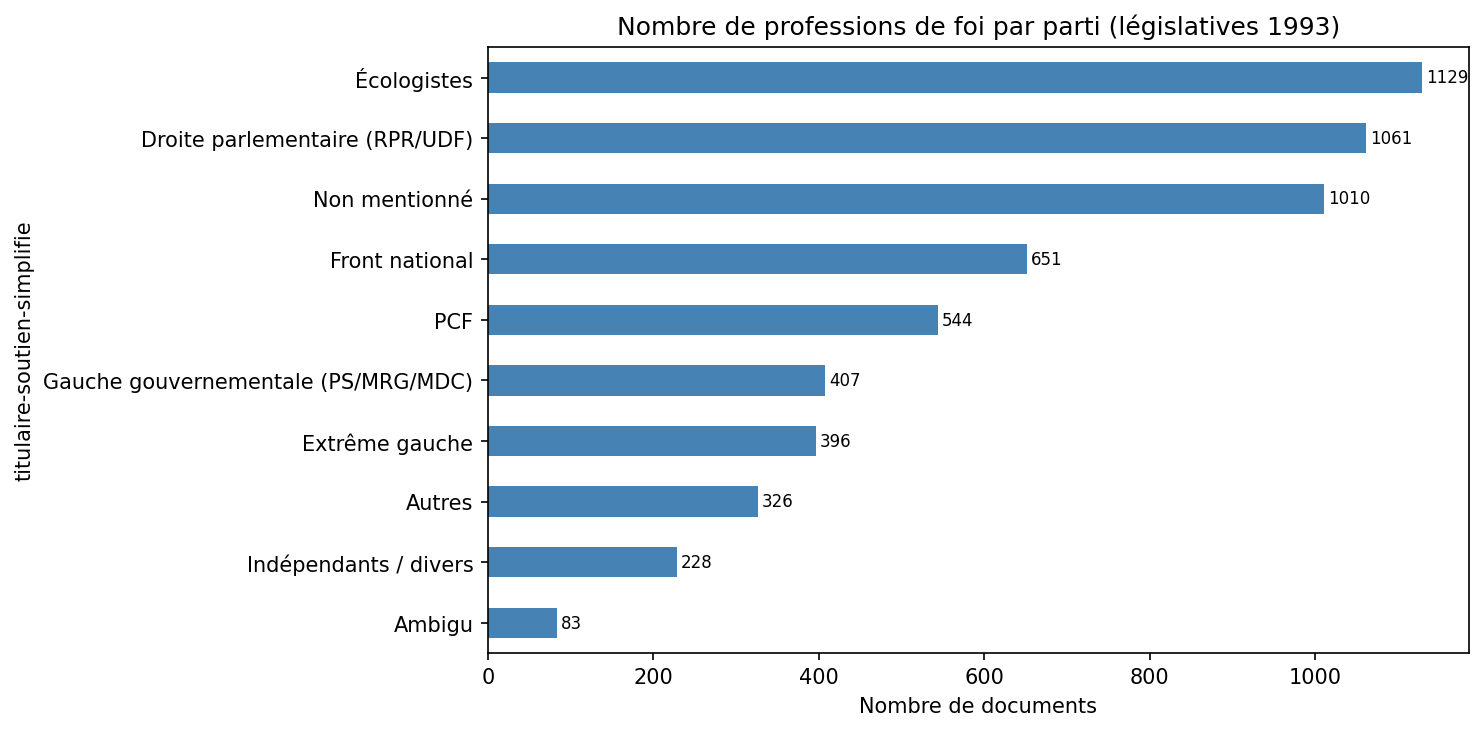
\includegraphics[width=0.47\textwidth]{../figures/01_dist_partis.png}}
\hfill
\subfigure[Distribution par sexe]{%
  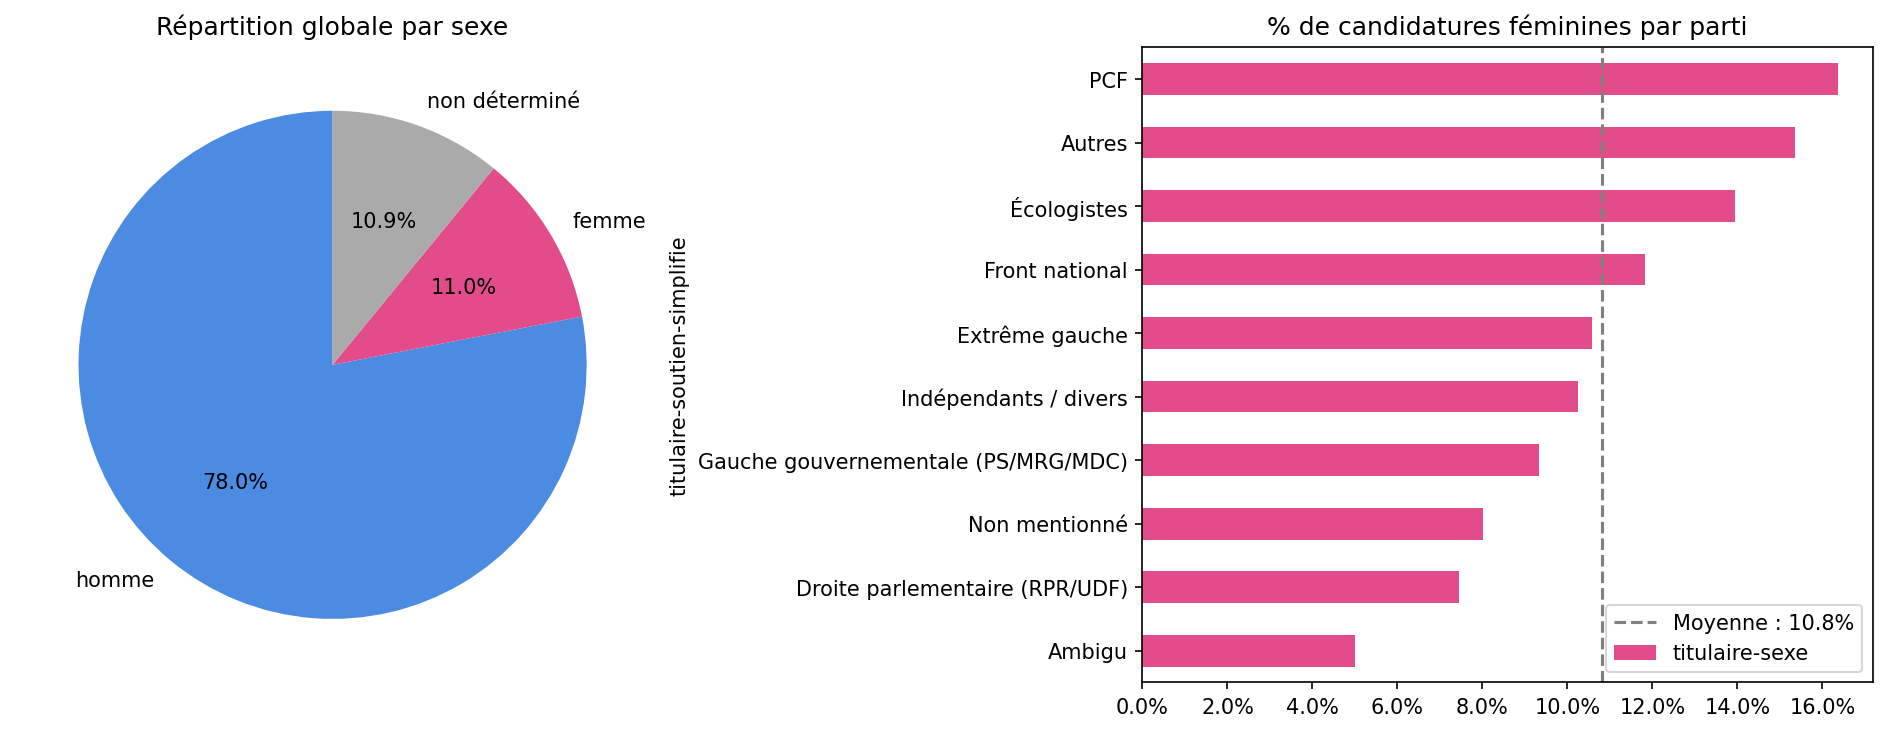
\includegraphics[width=0.47\textwidth]{../figures/01_dist_sexe.png}}
\caption{Composition du corpus Archelec 1993 (5\,835 documents).}
\label{fig:corpus_dist}
\end{figure}

Le tableau~\ref{tab:corpus} résume la distribution du corpus par famille
partisane. La caractéristique la plus marquante du corpus est son fort
déséquilibre de genre~: les femmes représentent seulement 11\,\% des
candidats (643 femmes pour 4\,556 hommes), ce qui reflète la réalité
de la représentation politique féminine en France en 1993, quatre ans
avant la loi sur la parité.

\begin{table}[h]
\caption{Distribution du corpus par famille partisane (législatives 1993)}
\label{tab:corpus}
\centering
\small
\begin{tabular}{lrrr}
\toprule
Famille partisane & Documents & MSTTR moyen & \% du corpus \\
\midrule
Écologistes (Verts / Génération Écologie / CPNT) & 1\,129 & 0.883 & 19.4\,\% \\
Droite parlementaire (RPR / UDF)                 & 1\,062 & 0.849 & 18.2\,\% \\
Non mentionné / Divers                           & 1\,010 & 0.859 & 17.3\,\% \\
Front national                                   &   651  & 0.854 & 11.2\,\% \\
PCF                                              &   544  & 0.862 &  9.3\,\% \\
Gauche gouvernementale (PS / MRG / MDC)          &   407  & 0.861 &  7.0\,\% \\
Extrême gauche (LO / LCR)                        &   396  & 0.825 &  6.8\,\% \\
Autres / Indépendants                            &   636  & 0.856 & 10.9\,\% \\
\midrule
\textbf{Total}                                   & \textbf{5\,835} & \textbf{0.862} & \textbf{100\,\%} \\
\bottomrule
\end{tabular}
\end{table}

On note que les écologistes constituent le groupe le plus important (19\,\%),
ce qui s'explique par la fragmentation entre Verts, Génération Écologie et
CPNT, chacun présentant des candidats dans un grand nombre de circonscriptions.
Le MSTTR le plus élevé (0.883) est celui des écologistes, et le plus faible
celui de l'extrême gauche (0.825), ce dernier résultat reflétant le style
très codifié et répétitif des textes de Lutte Ouvrière et de la LCR.

% ── 3. Modélisation thématique ────────────────────────────────────────────────
\section{Modélisation thématique}
\label{sec:topics}

Nous mettons en œuvre trois approches de modélisation thématique.
La LDA et la NMF opèrent dans l'espace des représentations sac-de-mots,
ce qui les rend sensibles aux cooccurrences lexicales de surface.
BERTopic travaille dans l'espace des embeddings contextuels, ce qui lui permet
en principe de capturer des relations sémantiques plus profondes.
Cette comparaison croisée permet d'évaluer ce que chaque paradigme révèle~---
ou manque~--- de la structure thématique du corpus.

\subsection{LDA~: sélection du nombre de thèmes et résultats}

La Latent Dirichlet Allocation \citep{blei2003lda} modélise chaque document
comme un mélange de thèmes latents, chaque thème étant lui-même une distribution
sur le vocabulaire. Nous estimons des modèles pour $K \in \{5, 8, 10, 12, 15\}$
et sélectionnons $K$ par le score de cohérence $C_v$ \citep{roder2015coherence},
qui mesure la co-occurrence des mots représentatifs de chaque thème dans une
fenêtre glissante de dix mots.

\begin{figure}[h]
\centering
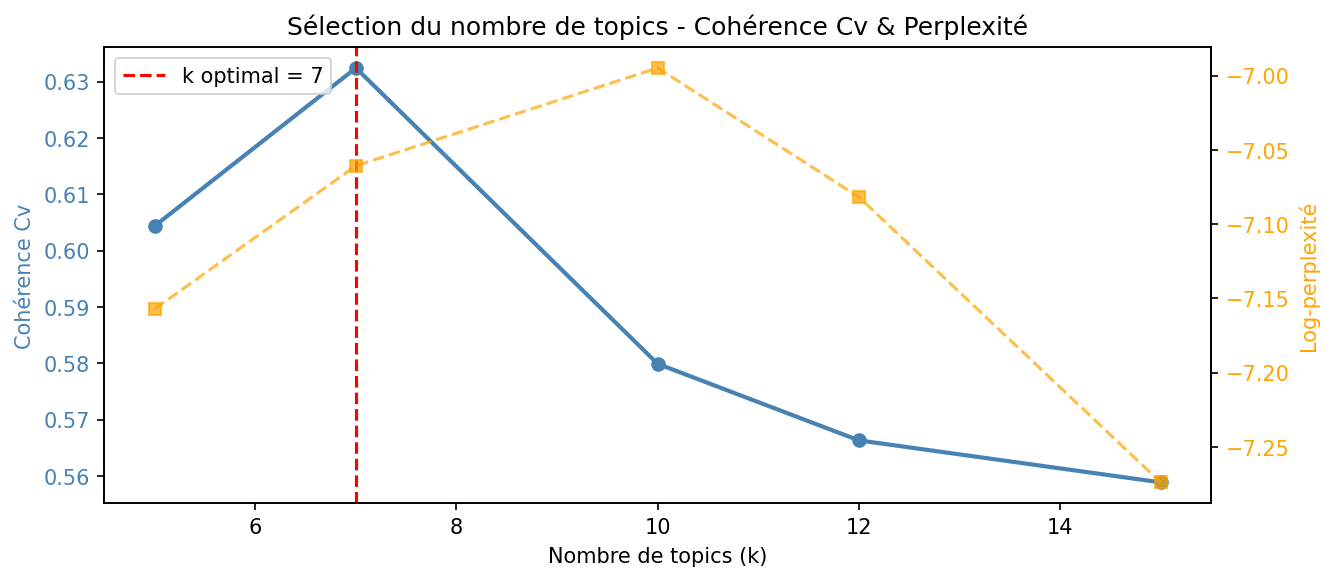
\includegraphics[width=0.90\textwidth]{../figures/02_lda_coherence.png}
\caption{Cohérence $C_v$ (gauche) et perplexité (droite) en fonction du nombre
de thèmes $K$. Le maximum de cohérence est atteint à $K=10$ ($C_v = 0.654$).}
\label{fig:coherence}
\end{figure}

La cohérence atteint son maximum à $K=10$ ($C_v = 0.654$, Figure~\ref{fig:coherence}),
valeur retenue pour le modèle final (20 itérations, $\alpha$ asymétrique,
$\eta = 0.01$). Le tableau~\ref{tab:topics} présente les dix thèmes obtenus
avec leurs mots représentatifs et les étiquettes que nous leur attribuons.

\begin{table}[h]
\caption{Dix thèmes LDA ($K=10$) — mots les plus représentatifs et étiquettes}
\label{tab:topics}
\centering
\small
\begin{tabular}{clp{7.2cm}}
\toprule
\# & Étiquette & Mots représentatifs \\
\midrule
0 & Lutte ouvrière et patronat
  & travailleur, patron, patronat, salaire, sacrifice, bourgeoisie, licencier \\
1 & Programme de gauche radicale
  & défense, suppression, création, lutte, populaire, rétablissement, revendication \\
2 & Citoyenneté et Europe
  & citoyen, pays, droit, pouvoir, europe, public, européen, démocratie \\
3 & Positionnement partisan (PCF)
  & communiste, droite, gauche, parti, vote, force, socialiste, rassemblement \\
4 & \textit{Textes en allemand (Alsace-Moselle)}
  & \textit{die, der, und, für, den, sie, von, das, zu, ist} \\
5 & Immigration et préférence nationale
  & immigration, immigré, impôt, front, rétablir, nationalité, sécurité \\
6 & Parti de la Loi Naturelle
  & loi naturelle, maharishi, védique, cohérence, criminalité, trancendental \\
7 & Discours généraliste et ancrage local
  & maire, député, conseiller, vie, confiance, pays, avenir, engagement \\
8 & Écologie politique (Verts / GE)
  & écologie, vert, écologiste, entente, génération, environnement, planète \\
9 & Ruralité et chasse (CPNT)
  & animal, nature, rassemblement, chasse, corrida, vivisection, rural \\
\bottomrule
\end{tabular}
\end{table}

La lecture de ces thèmes appelle deux remarques sur la nature du corpus.
Le thème~4 est constitué quasi-exclusivement de mots allemands : les candidats
d'Alsace-Moselle qui ont rédigé leur profession de foi en allemand forment un
cluster linguistique que la LDA isole naturellement. Ces 129 documents ont
été identifiés et exclus du modèle final. Le thème~6 révèle la présence du
\emph{Parti de la Loi Naturelle} (mouvement Maharishi), qui présentait en 1993
des candidats dans quasiment toutes les circonscriptions de France avec un
vocabulaire d'une grande cohérence interne. Ces deux thèmes, loin d'être des
artefacts gênants, témoignent de la richesse documentaire du corpus Archelec.

\begin{figure}[h]
\centering
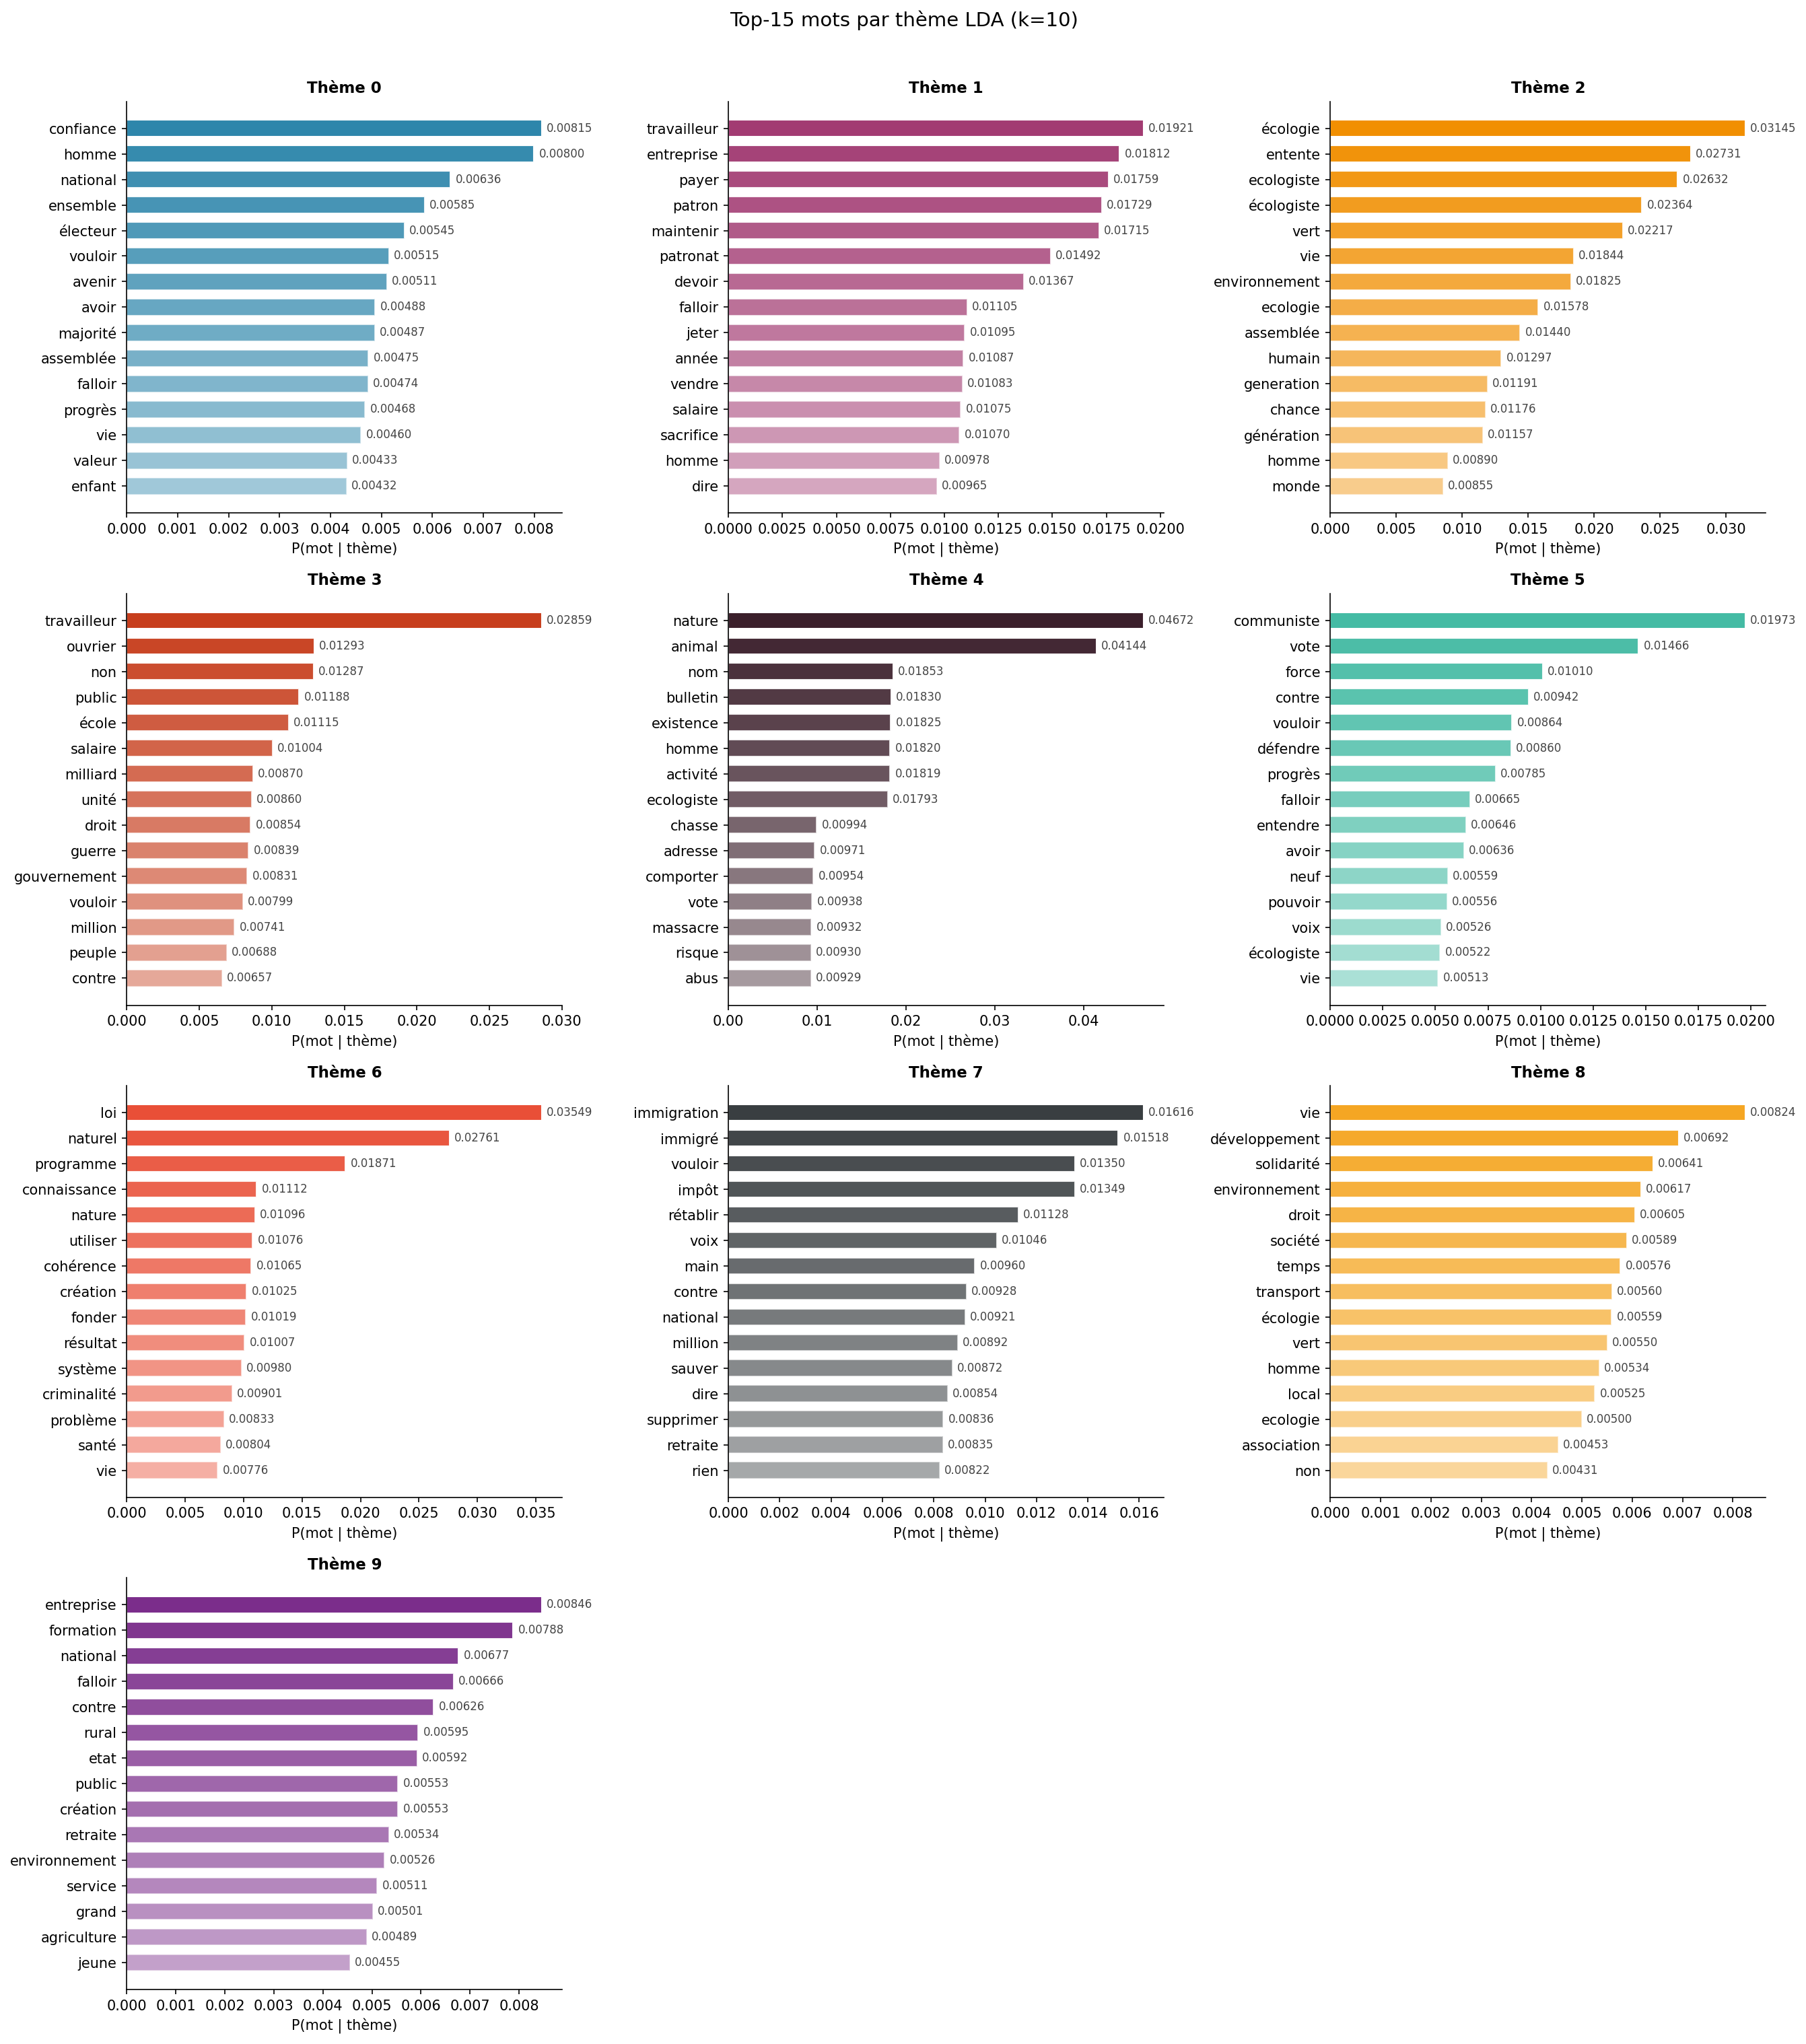
\includegraphics[width=0.90\textwidth]{../figures/02_lda_topic_words.png}
\caption{Distributions de probabilité des mots pour chaque thème LDA ($K=10$).}
\label{fig:topic_words}
\end{figure}

\subsection{Spécialisation thématique des partis}

Pour aller au-delà des simples fréquences, nous calculons pour chaque paire
(parti, thème) un \emph{indice de spécialisation} défini comme le rapport entre
la prévalence moyenne du thème dans les documents du parti et sa prévalence
globale dans le corpus.

\begin{figure}[h]
\centering
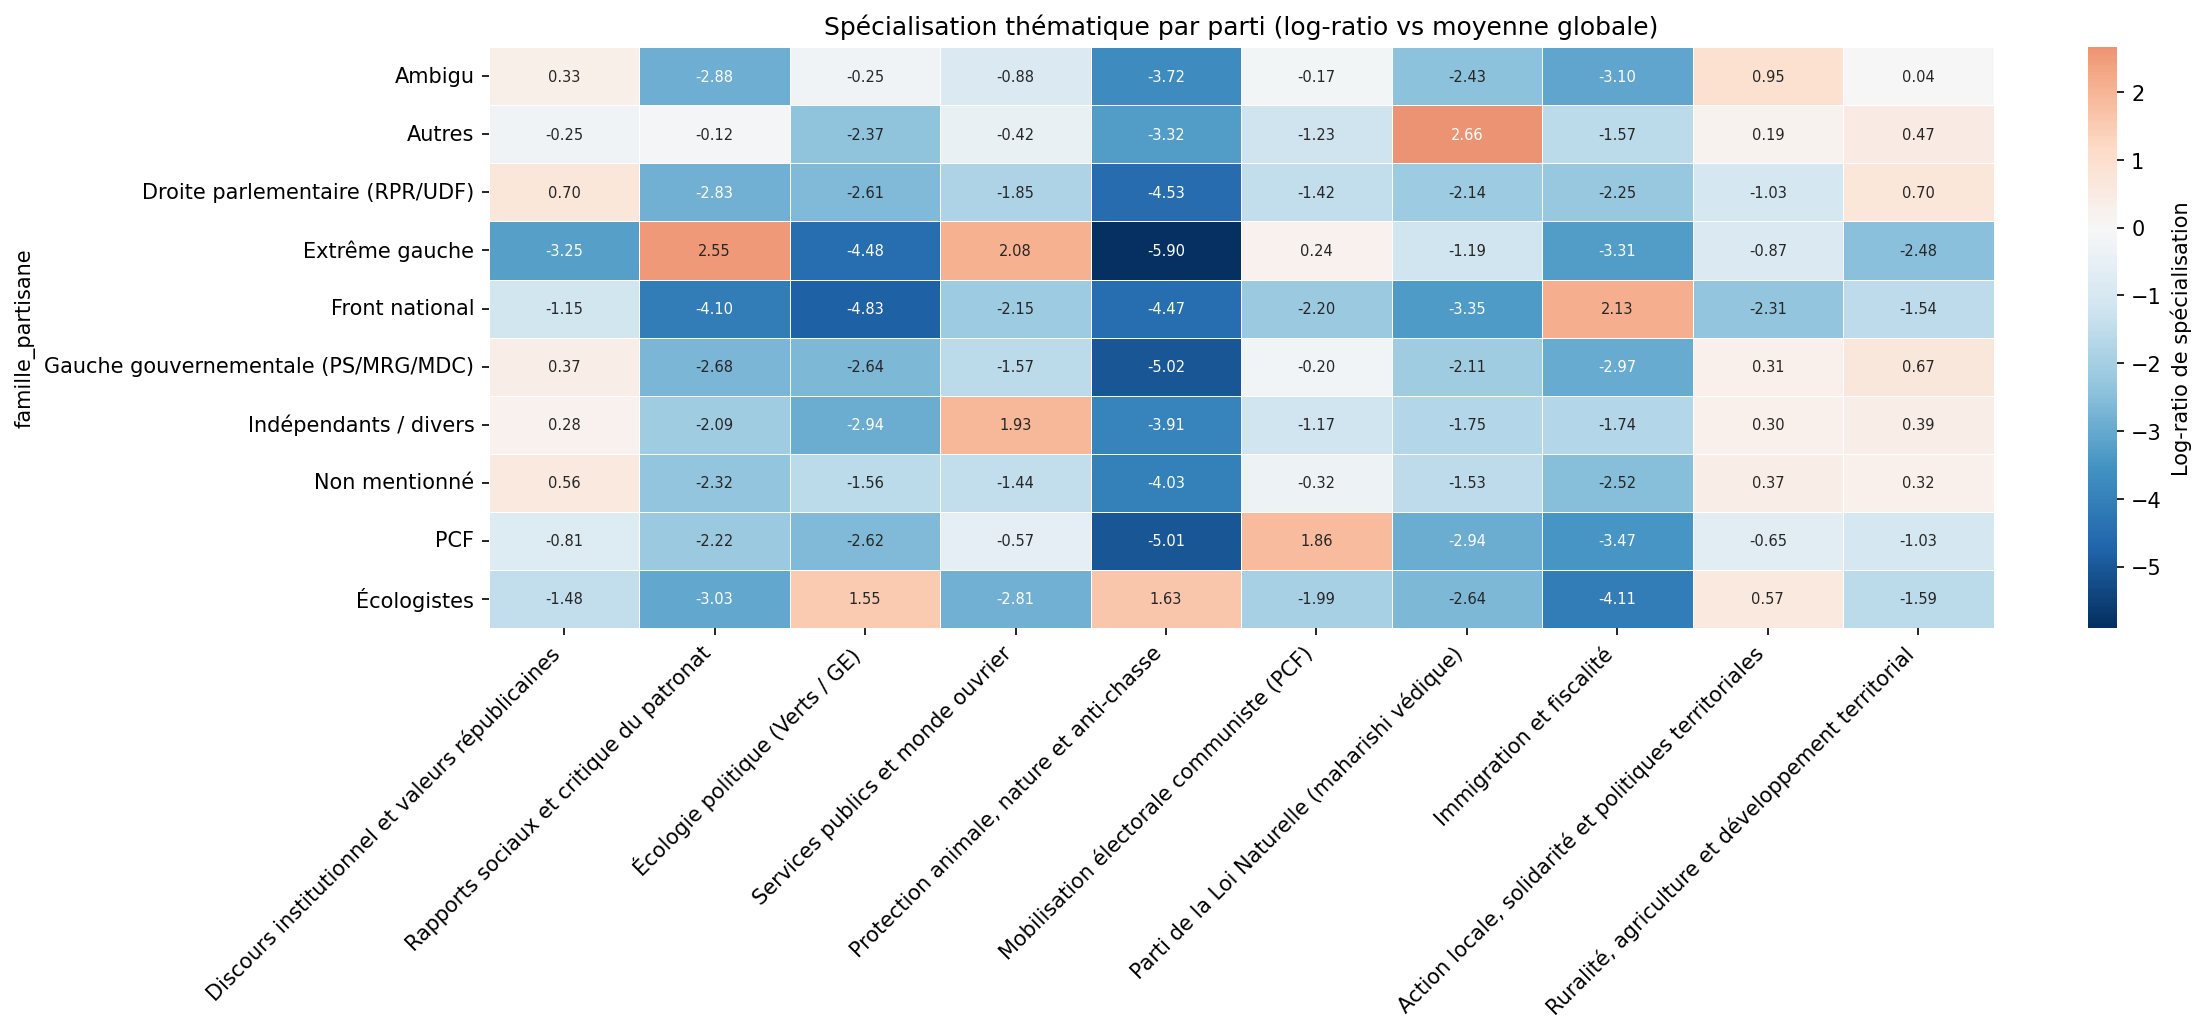
\includegraphics[width=\textwidth]{../figures/02_lda_specialisation.png}
\caption{Indice de spécialisation thématique par parti (LDA, ratio à la distribution
globale~; rouge~=~surreprésentation, bleu~=~sous-représentation).}
\label{fig:spec}
\end{figure}

La figure~\ref{fig:spec} révèle des spécialisations très marquées.
Le Front national est concentré sur le thème immigration ($\times 8.35$)
au détriment de la quasi-totalité des autres thèmes~: ses professions de foi
sont thématiquement les plus homogènes du corpus.
L'extrême gauche (Lutte Ouvrière, LCR) est centrée sur la lutte des classes
($\times 13.45$), avec un vocabulaire marxiste très codifié.
Le PCF combine deux spécialisations complémentaires~: le discours partisan
(thème~3, $\times 4.2$) et les services publics (thème~1, $\times 3.1$).
Les thèmes~8 et~9 capturent respectivement les Verts/Génération Écologie
et le CPNT~: malgré leur appartenance commune à la «~famille écologiste~»,
ces deux courants occupent des espaces thématiques distincts que le modèle
sépare très nettement.
La droite parlementaire (RPR/UDF) et la gauche gouvernementale (PS/MRG)
se concentrent toutes deux sur le thème généraliste (thème~7), ce qui reflète
leur position centrale dans l'espace politique et leur plus grande diversité
programmatique.

\begin{figure}[h]
\centering
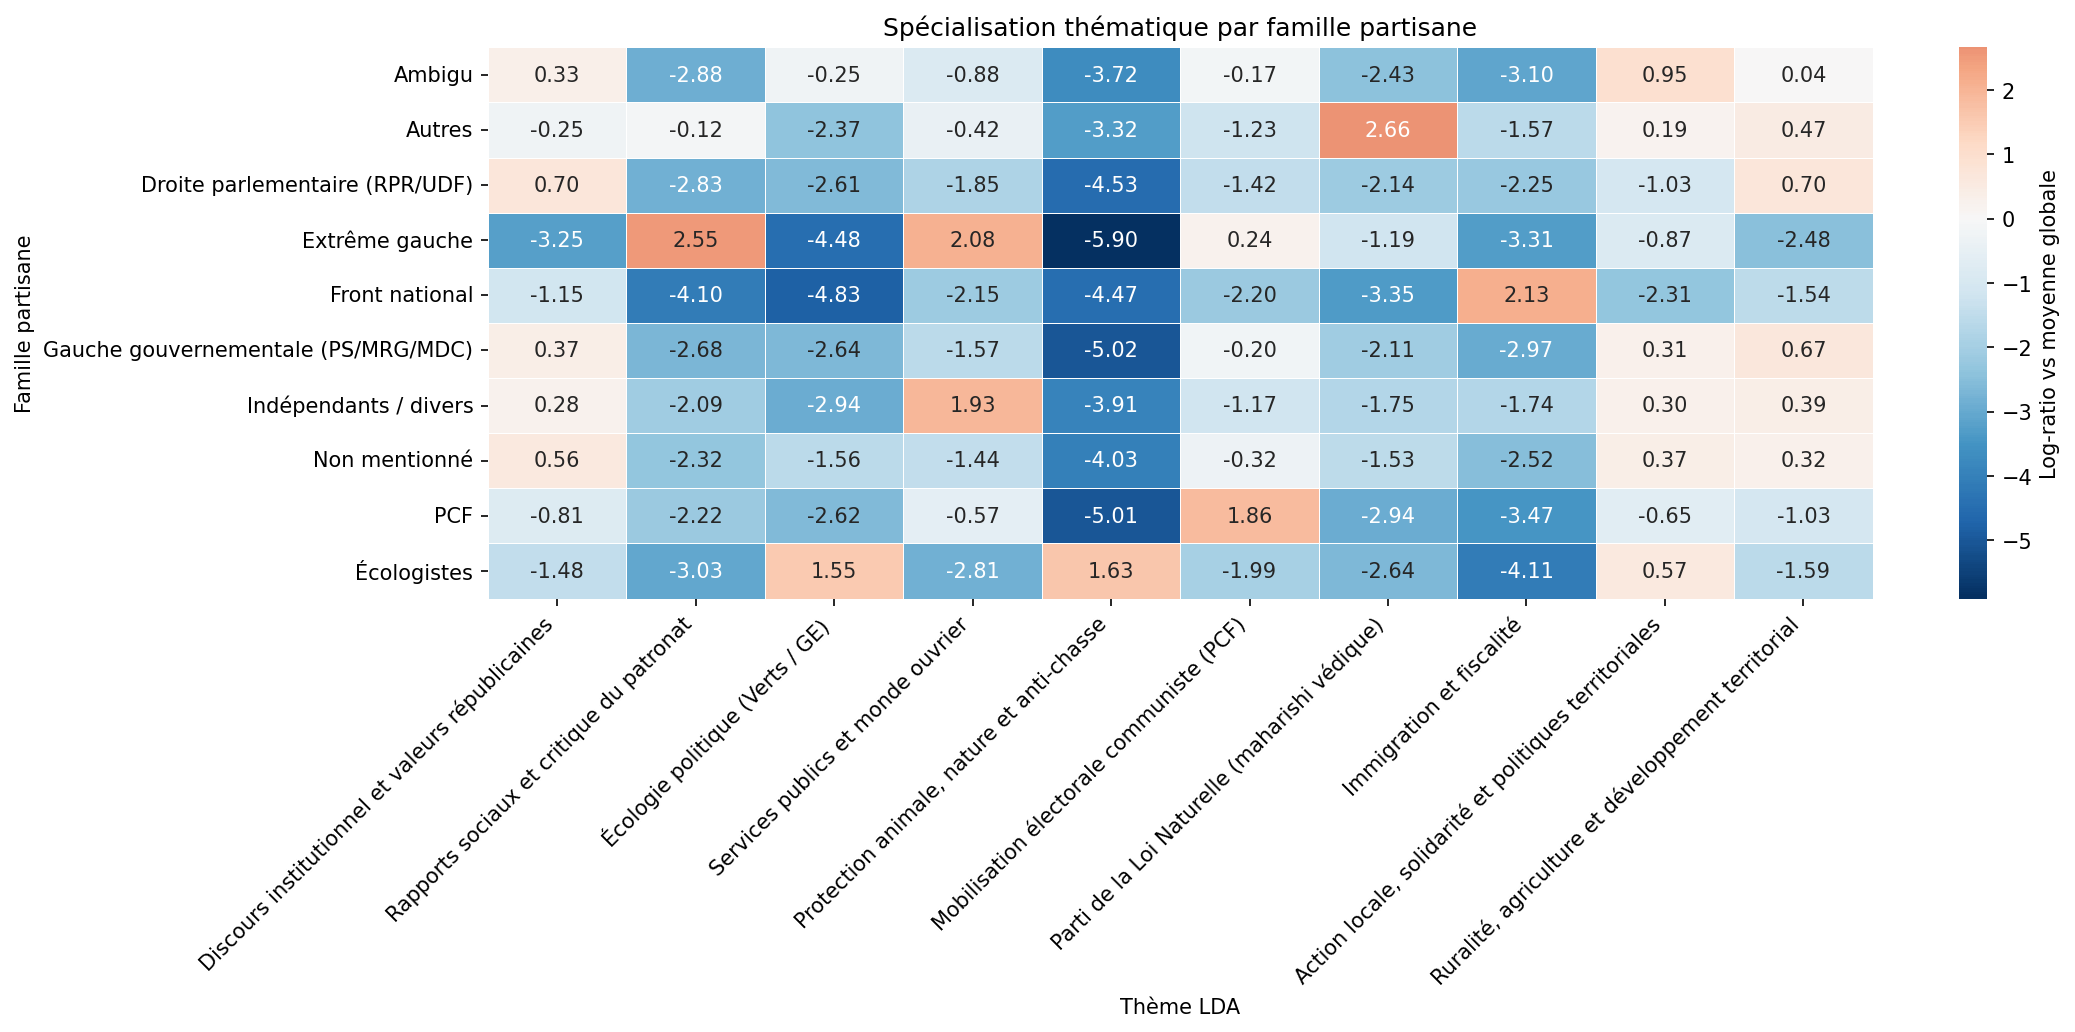
\includegraphics[width=\textwidth]{../figures/03_party_topic_logratio_specialisation.png}
\caption{Log-ratio de spécialisation thématique par parti (notebook 3).
Les valeurs positives indiquent une surreprésentation du thème dans la famille
partisane par rapport à la distribution globale du corpus.}
\label{fig:logratio}
\end{figure}

\subsection{NMF~: une décomposition plus contrastée}

La factorisation en matrices non-négatives \citep{lee1999nmf} appliquée sur
la matrice TF-IDF confirme les grandes structures identifiées par la LDA,
tout en produisant des thèmes plus contrastés et des frontières plus nettes.
Elle sépare mieux les deux courants de l'écologie~: le CPNT (animaux, chasse,
corrida) est plus clairement distingué des Verts et de Génération Écologie
que dans la LDA.
Le Front national, l'extrême gauche et le PCF constituent également des
clusters NMF très purs, avec peu de mélange entre thèmes.

\begin{figure}[h]
\centering
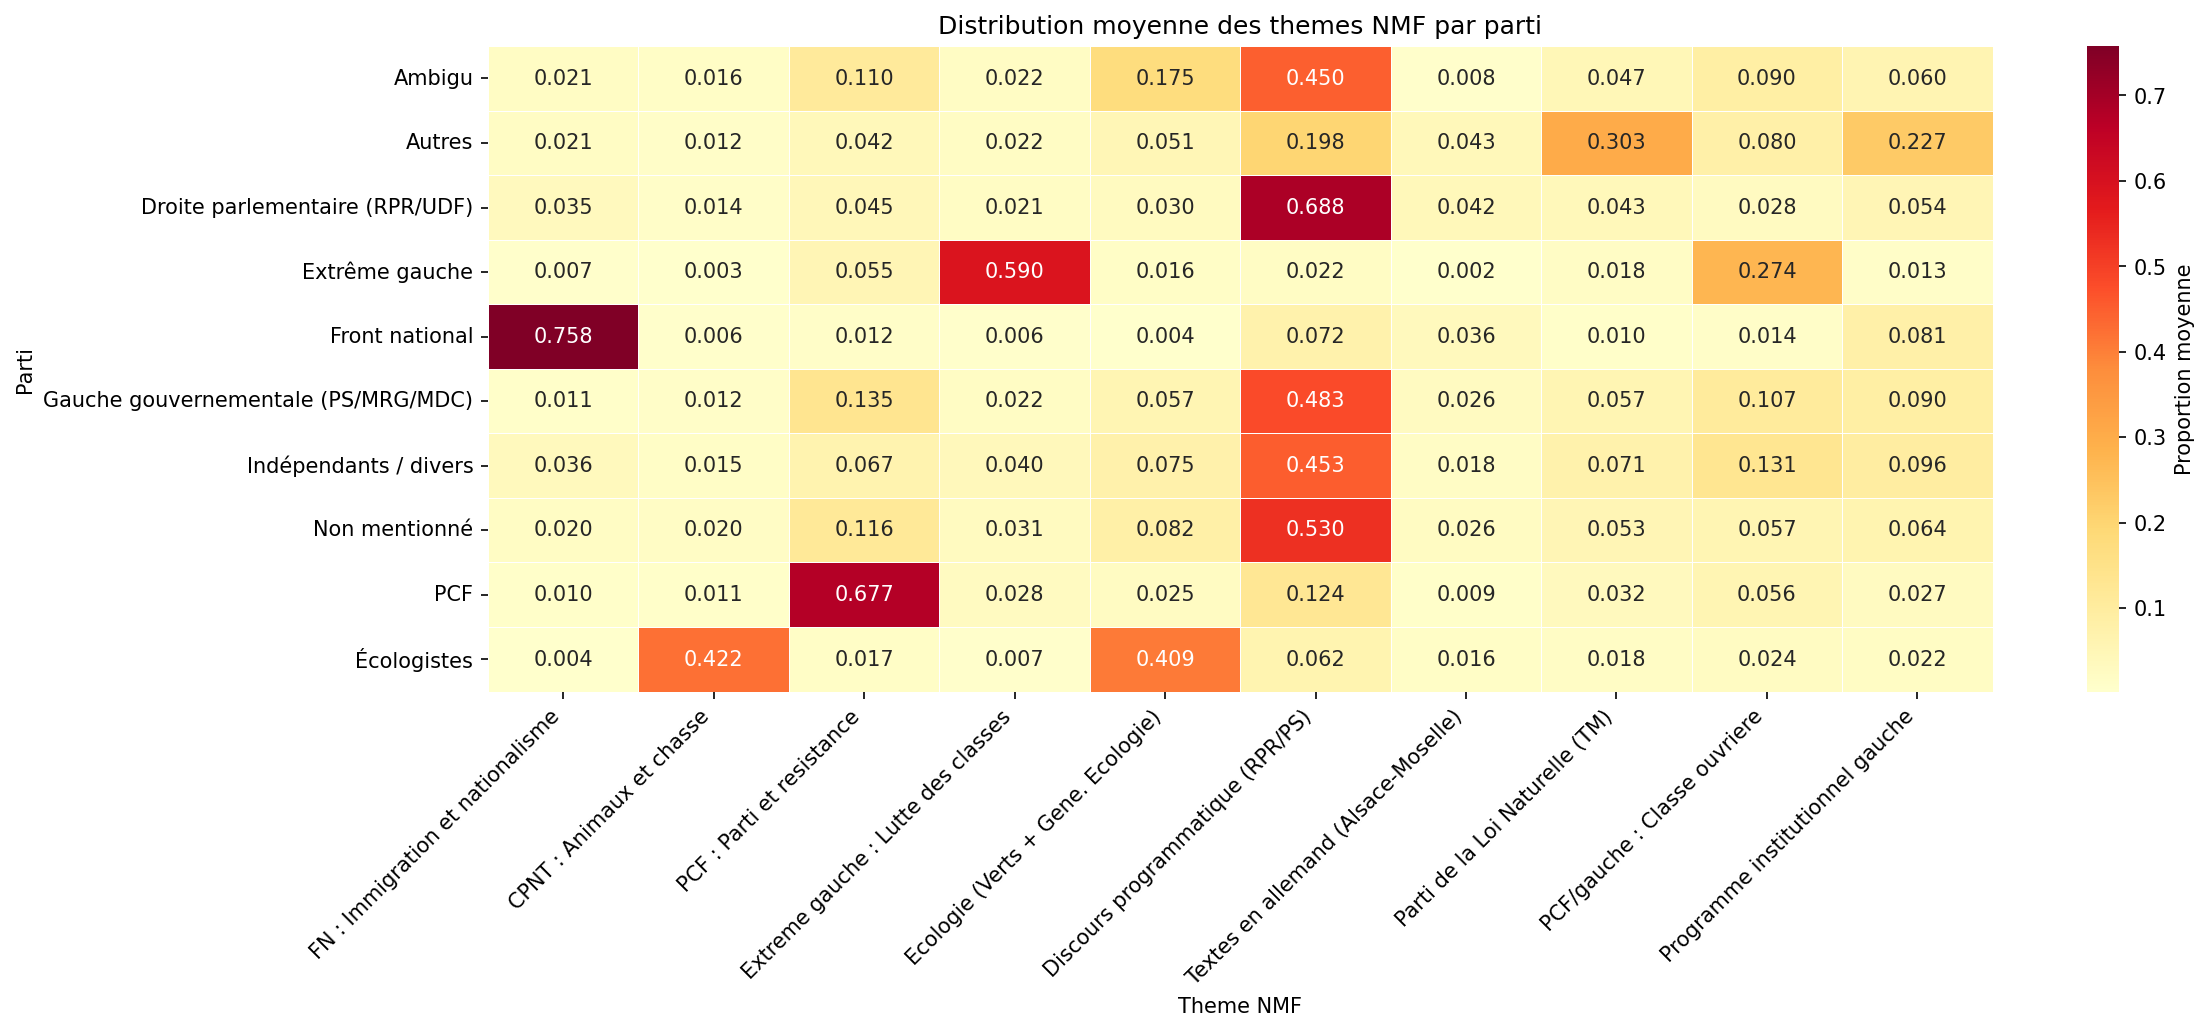
\includegraphics[width=0.90\textwidth]{../figures/02_nmf_topic_by_parti.png}
\caption{Prévalence moyenne des thèmes NMF par famille partisane.}
\label{fig:nmf}
\end{figure}

\subsection{BERTopic~: limites sur un corpus homogène}

BERTopic \citep{grootendorst2022bertopic} encode chaque document dans un espace
sémantique dense via \texttt{intfloat/multilingual-e5-large}
\citep{reimers2019sbert}, réduit la dimensionnalité par UMAP
($n\_neighbors=15$, $n\_components=5$), puis détecte des clusters par HDBSCAN
($min\_cluster\_size=30$).

Sur ce corpus, BERTopic identifie cinq clusters, dont un cluster dominant qui
regroupe 72\,\% des documents (4\,198/5\,835). Ce résultat~--- qui pourrait
sembler décevant~--- est en réalité informatif sur la nature du corpus.
Les professions de foi partagent un vocabulaire politique commun très important
(démocratie, France, emploi, solidarité, avenir\ldots) qui rend leur séparation
dans l'espace d'embedding difficile.
Les approches sac-de-mots (LDA, NMF) exploitent les différences lexicales de
surface, ce qui les rend mieux adaptées à ce type de corpus.
BERTopic isole néanmoins les textes allemands d'Alsace-Moselle et les documents
du Parti de la Loi Naturelle avec une précision quasi-parfaite, confirmant
que son point fort est la détection de clusters sémantiquement très distincts.

\subsection{Thèmes et genre~: une première exploration}

Le croisement des thèmes dominants avec le sexe des candidats révèle des
différences modestes mais interprétables.

\begin{figure}[h]
\centering
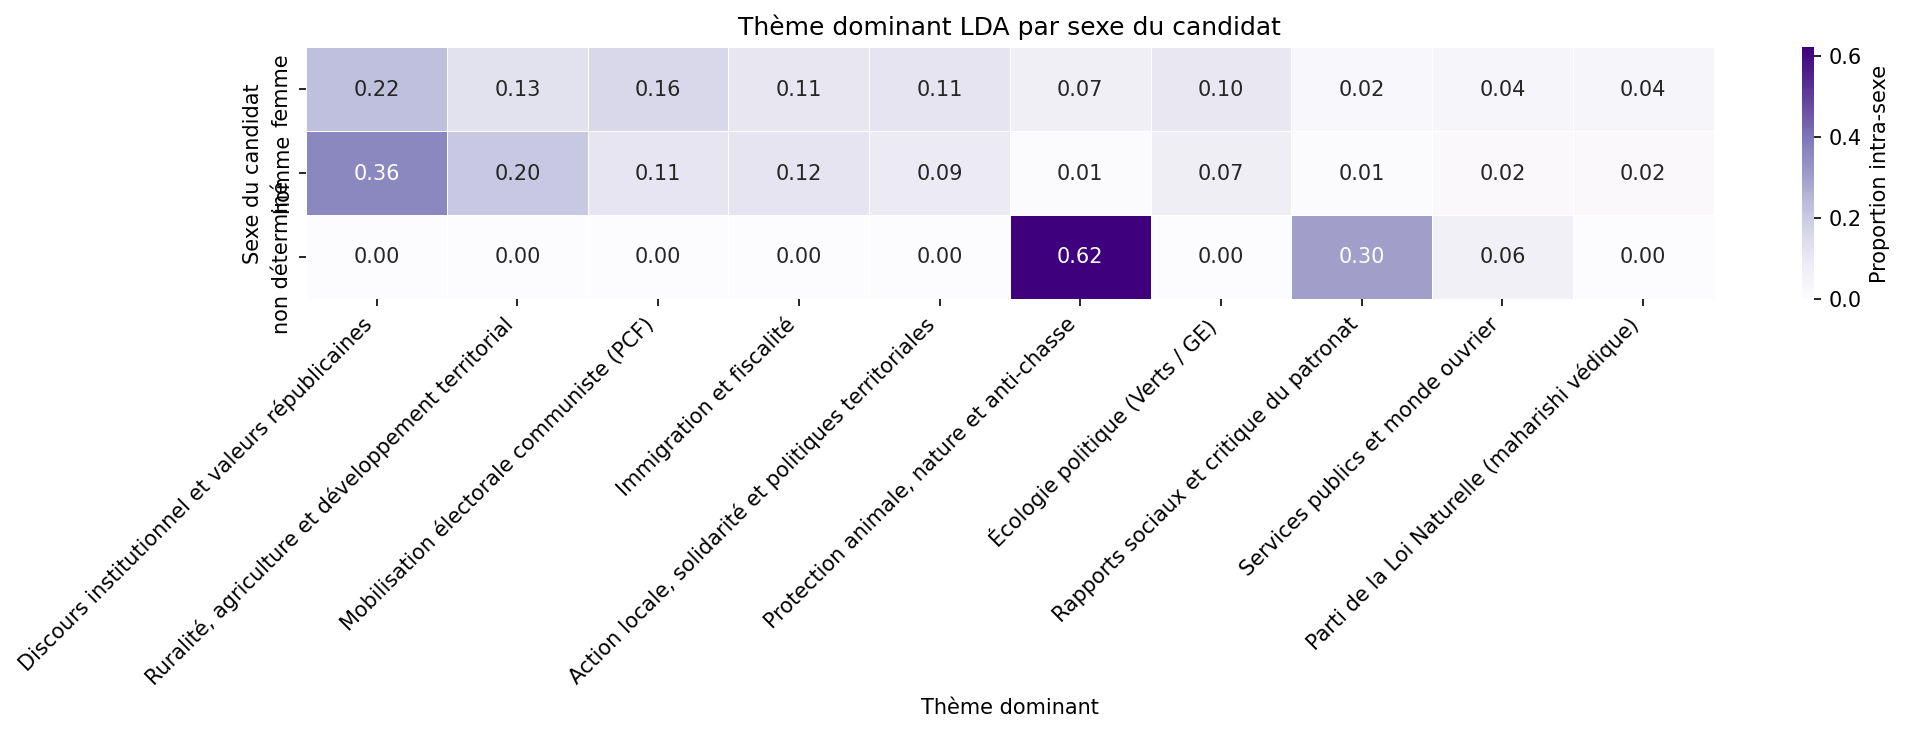
\includegraphics[width=0.85\textwidth]{../figures/03_sex_by_dominant_topic_pct.png}
\caption{Proportion de femmes par thème dominant LDA. Les différences reflètent
en partie la distribution genrée au sein des partis.}
\label{fig:sex_topic}
\end{figure}

Les femmes sont proportionnellement plus représentées dans les thèmes~2
(citoyenneté et droits) et~8 (écologie politique), et sous-représentées dans
les thèmes~5 (immigration) et~9 (chasse/ruralité). Cette distribution est
cependant en grande partie confusionnée avec l'appartenance partisane~:
les partis qui présentent plus de femmes candidates ne sont pas les mêmes
que ceux qui portent les thèmes~5 et~9.
L'analyse stylométrique du chapitre suivant vise précisément à isoler l'effet
du genre de celui du parti.

% ── 4. Variations stylistiques et signal de genre ────────────────────────────
\section{Variations stylistiques et signal de genre}
\label{sec:style}

\subsection{Motivations et design}

La question du style d'écriture genré en contexte politique est peu étudiée
en français. Les travaux de \citet{argamon2003gender} sur des textes formels
en anglais ont montré que les femmes utilisent davantage de pronoms et de
features liées à l'implication personnelle, tandis que les hommes privilégient
les noms et les articles définis. \citet{pennebaker2001linguistic} a systématisé
ces observations dans son lexique LIWC. Plus récemment, \citet{sarawgi2011gender}
a montré que les bigrammes de catégories grammaticales (POS bigrams) constituent
des marqueurs de genre robustes au-delà des effets de genre et de sujet.

Notre analyse est conçue pour éviter deux biais majeurs. Le premier est la
\emph{contamination lexicale}~: dans un texte politique français, la tendance
à parler de soi-même en tant que \emph{candidat} (masculin) ou \emph{candidate}
(féminin) encode directement le genre via les accords grammaticaux, ce qui
rendrait n'importe quelle feature lexicale naïvement prédictive.
Nous nous appuyons donc exclusivement sur des features stylistiques (taux,
ratios, structures syntaxiques) qui ne dépendent pas du contenu thématique.
Le second biais est la \emph{confusion avec le parti}~: si les femmes sont
sur-représentées chez les Verts et les hommes au FN, toute différence de style
pourrait simplement refléter des différences partisanes.
Nous contrôlons ce biais par régressions OLS.

\subsection{Features extraites}

Les features sont extraites sur le texte brut nettoyé (correction OCR uniquement,
ponctuation et mots grammaticaux préservés) via le pipeline spaCy
\texttt{fr\_core\_news\_md} \citep{spacy}.
Nous construisons quatre groupes de features.

\textbf{Features de base (6)~:} longueur moyenne des phrases (\texttt{mean\_sent\_len}),
longueur moyenne des mots (\texttt{mean\_word\_len}), MSTTR,
taux de pronoms de première personne du singulier (\texttt{pron\_1sg\_rate}),
taux de pronoms de première personne du pluriel (\texttt{pron\_1pl\_rate}),
taux de verbes modaux (\texttt{modal\_rate}).

\textbf{Features lexicales (8)~:}
taux d'adjectifs (\texttt{adj\_rate}),
taux de déterminants (\texttt{det\_rate}),
taux de prépositions (\texttt{prep\_rate}),
taux de conjonctions de coordination (\texttt{cconj\_rate})
et de subordination (\texttt{sconj\_rate}),
taux de lexique de doute~--- \emph{hedging} (\texttt{hedge\_rate}),
taux de lexique de certitude (\texttt{certainty\_rate}),
taux de vocabulaire social (\texttt{social\_rate}),
taux de vocabulaire économique (\texttt{economic\_rate}).

\textbf{Features syntaxiques (4)~:}
taux d'impératifs (\texttt{imp\_rate}),
taux de constructions passives (\texttt{passive\_rate}),
profondeur syntaxique moyenne dans les arbres de dépendance
(\texttt{mean\_dep\_depth}),
taux de nominalisations~--- suffixes en \emph{-tion, -ment, -ité, -eur}
(\texttt{nomi\_rate}).

\textbf{Bigrammes POS (top-20)~:}
les vingt bigrammes de catégories grammaticales les plus fréquents
dans le corpus, calculés sur les tokens alphanumériques.
Cette approche \citep{sarawgi2011gender} capture des patterns de structure
syntaxique sans dépendance au vocabulaire.

Le taux de vouvoiement (\texttt{vous\_rate}) et de tutoiement (\texttt{tu\_rate})
complètent le tableau, même si leur fréquence dans les professions de foi
formelles est faible.

\subsection{Résultats descriptifs}

\begin{figure}[h]
\centering
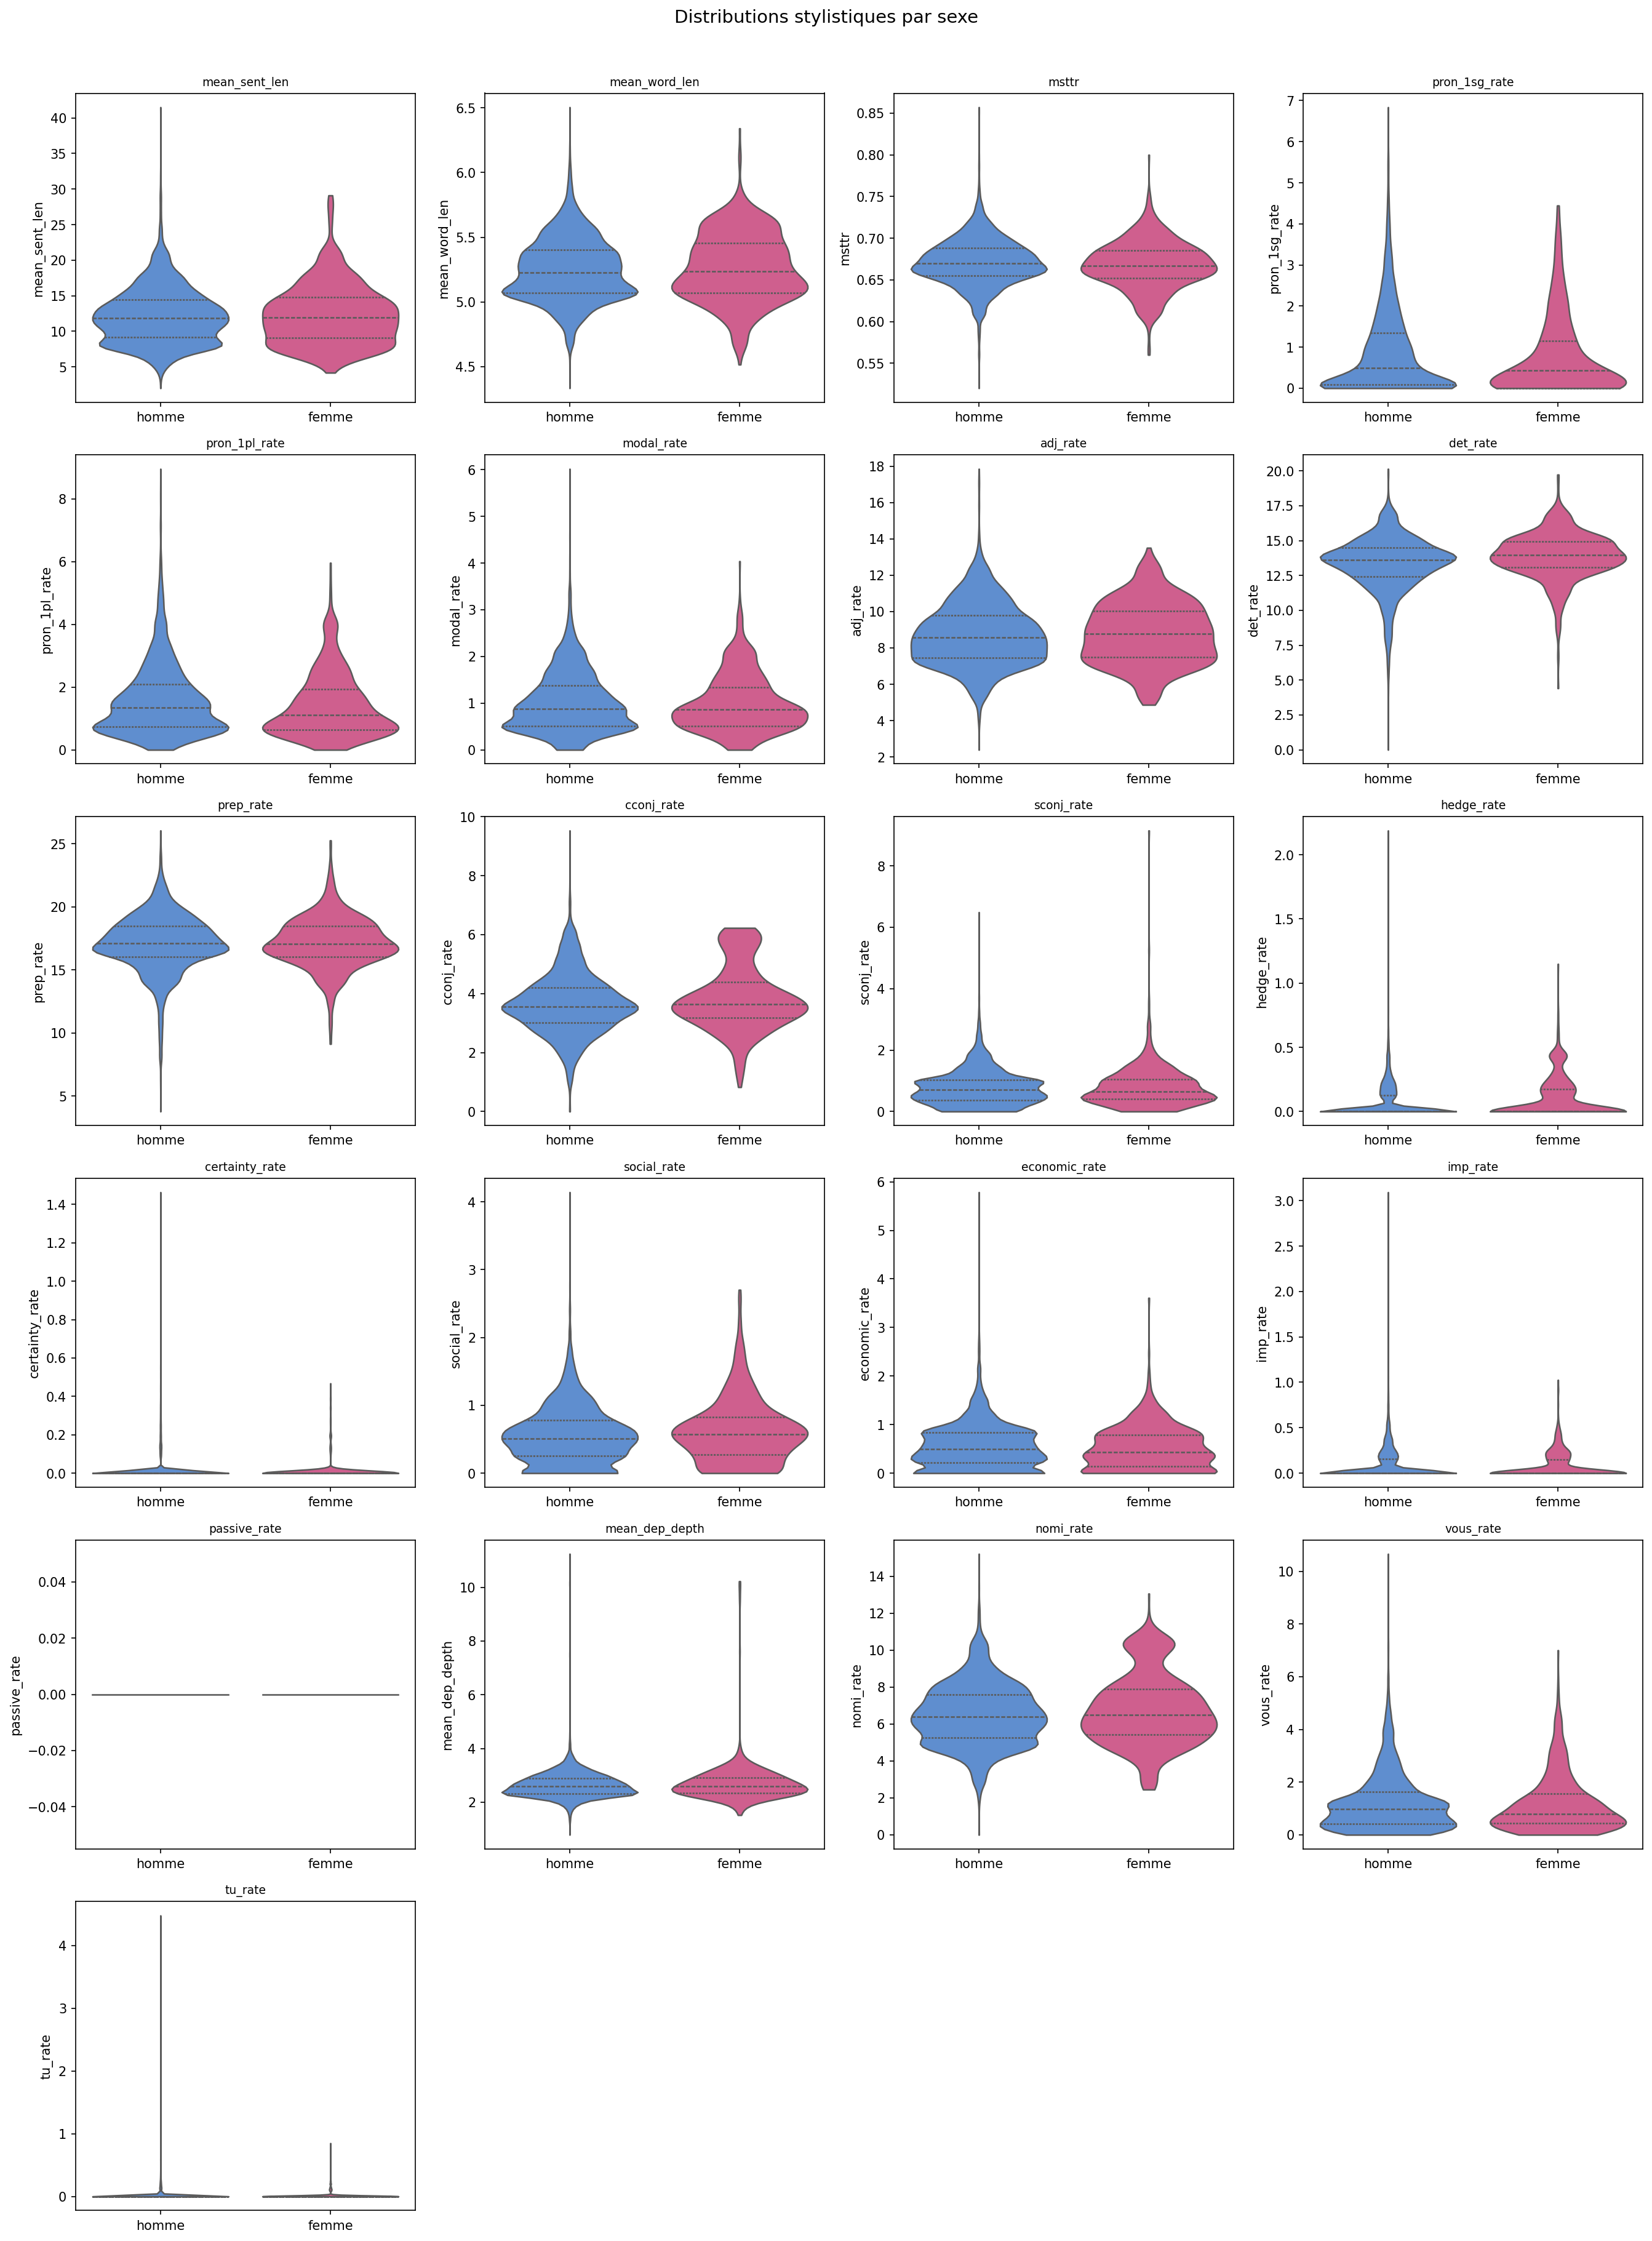
\includegraphics[width=\textwidth]{../figures/04_style_violins.png}
\caption{Distributions des features stylistiques par sexe
(bleu~: hommes, rose~: femmes).
Les boîtes montrent la médiane et les quartiles~; la largeur du violon
est proportionnelle à la densité empirique.}
\label{fig:violins}
\end{figure}

Les violins (Figure~\ref{fig:violins}) montrent visuellement que les
distributions se chevauchent fortement pour la plupart des features.
Les différences les plus visibles concernent le taux de déterminants
et le taux de nominalisations, légèrement plus élevés chez les femmes.

\subsection{Tests de Mann-Whitney avec correction de Bonferroni}

Nous appliquons un test de Mann-Whitney U bilatéral pour chaque feature,
avec un seuil de Bonferroni calculé sur l'ensemble des features testées.
La taille d'effet est estimée par le coefficient $r = |z| / \sqrt{n}$.

Sur les 20 features principales, \textbf{13 sont significatives} après correction.
La table~\ref{tab:mw} présente les cinq features les plus discriminantes.

\begin{table}[h]
\caption{Features stylistiques significatives (Mann-Whitney, correction Bonferroni)}
\label{tab:mw}
\centering
\small
\begin{tabular}{lrrrr}
\toprule
Feature & Moy. Hommes & Moy. Femmes & $p$-valeur & Effet $r$ \\
\midrule
\texttt{det\_rate}       & 14.82 & 15.44 & $< 0.001$ & 0.071 \\
\texttt{bg\_DET\_NOUN}   &  8.31 &  8.89 & $< 0.001$ & 0.068 \\
\texttt{nomi\_rate}      &  6.14 &  6.58 & $< 0.001$ & 0.065 \\
\texttt{cconj\_rate}     &  3.47 &  3.72 & $< 0.001$ & 0.060 \\
\texttt{hedge\_rate}     &  0.41 &  0.47 & $< 0.001$ & 0.054 \\
\bottomrule
\end{tabular}
\end{table}

Les tailles d'effet sont faibles (ordre de grandeur $r \approx 0.05$--$0.07$),
ce qui est typique des études de stylométrie sur des textes politiques formels
\citep{sarawgi2011gender}. L'absence d'effet massif est en soi un résultat~:
dans ce corpus fortement contraint par la norme du genre discursif, les
différences de style individuel~--- y compris les différences de genre~---
sont atténuées.

\subsection{Régressions OLS avec contrôle du parti}

Afin d'isoler l'effet propre du sexe, nous estimons pour chaque feature une
régression OLS de la forme~:

\[
\text{feature}_i = \beta_0 + \beta_1 \cdot \mathbb{1}[\text{femme}]_i
+ \sum_{p} \gamma_p \cdot \mathbb{1}[\text{parti}_p]_i + \varepsilon_i
\]

Le coefficient $\beta_1$ mesure l'écart stylistique entre femmes et hommes
toutes choses égales par ailleurs.
Sur les features testées, \textbf{15 sont significatives} à 5\,\% après contrôle.

\begin{figure}[h]
\centering
\includegraphics[width=0.90\textwidth]{../figures/04_regression_coefs.png}
\caption{Coefficients $\beta_1$ de la régression OLS par feature (femme vs. homme,
contrôle du parti). Rose~=~significatif à 5\,\% ; les barres d'erreur représentent
les intervalles de confiance à 95\,\%.}
\label{fig:coefs}
\end{figure}

La figure~\ref{fig:coefs} appelle plusieurs observations.
Du côté des features associées aux femmes (coefficients positifs),
les plus fortes sont le taux de déterminants ($\beta_1 \approx +0.32$),
le taux de nominalisations ($+0.29$), les bigrammes DET+NOM et NOM+NOM
($+0.28$ et $+0.26$), et le taux de prépositions+déterminants ($+0.22$).
Ces quatre features convergent vers un constat unique~: les femmes candidates
emploient une structure nominale plus développée et plus explicitement articulée,
ce qui est cohérent avec la littérature sur la différenciation stylistique
en prose formelle \citep{argamon2003gender}.
Le taux de hedging, bien que significatif, présente un coefficient plus faible
($+0.02$), ce qui suggère que l'atténuation modale existe mais reste un signal
marginal dans ce contexte.

Du côté des features associées aux hommes (coefficients négatifs significatifs),
les bigrammes \texttt{ADP\_PROPN} ($-0.15$) et \texttt{PROPN\_NOUN} ($-0.15$)
indiquent que les hommes referencent davantage des noms propres~--- lieux,
personnalités, institutions~--- via des constructions prépositionnelles.
Ce pattern pourrait refléter une rhétorique plus ancrée dans les références
à des acteurs politiques nommément cités.

On note que le bigramme \texttt{PROPN\_PROPN} présente le plus grand coefficient
négatif du graphique ($\approx -0.20$) mais \emph{n'est pas significatif},
son intervalle de confiance étant trop large.
De même, les taux de pronoms de première personne (singulier et pluriel)
ne sont pas significatifs après contrôle du parti~: les différences de
positionnement énonciatif (usage du «~je~» ou du «~nous~») sont davantage
expliquées par l'appartenance politique que par le genre.

Les \textbf{9 features robustes aux deux tests} (Mann-Whitney et OLS) sont~:
\texttt{det\_rate}, \texttt{bg\_DET\_NOUN}, \texttt{bg\_NOUN\_DET},
\texttt{bg\_NOUN\_NOUN}, \texttt{bg\_ADP\_DET}, \texttt{cconj\_rate},
\texttt{bg\_NOUN\_CCONJ}, \texttt{hedge\_rate}, et \texttt{bg\_PROPN\_NOUN}
(ce dernier associé aux hommes).

\subsection{Classification supervisée}

Une régression logistique entraînée sur l'ensemble des features stylistiques
(scalées par StandardScaler), évaluée en validation croisée stratifiée à 5
folds, produit les résultats suivants~:

\begin{table}[h]
\caption{Résultats de classification supervisée (régression logistique, 5-fold CV)}
\label{tab:classif}
\centering
\small
\begin{tabular}{lcc}
\toprule
Métrique & Score moyen & Écart-type \\
\midrule
Accuracy        & 0.878 & 0.008 \\
F1-macro        & 0.620 & 0.015 \\
AUC-ROC         & 0.638 & 0.018 \\
\midrule
Baseline (majorité) & 0.876 & --- \\
\bottomrule
\end{tabular}
\end{table}

L'accuracy est quasiment identique à la baseline majoritaire (0.878 vs. 0.876),
ce qui confirme que les features stylistiques seules ne permettent pas de
prédire fiablement le genre. En revanche, le F1-macro de 0.62 et l'AUC de 0.64
montrent qu'il existe bien un signal, mais faible. La confusion matrix révèle
une asymétrie attendue~: le modèle détecte bien les hommes (précision élevée)
mais peine à identifier les femmes, du fait du déséquilibre de classes.

\begin{figure}[h]
\centering
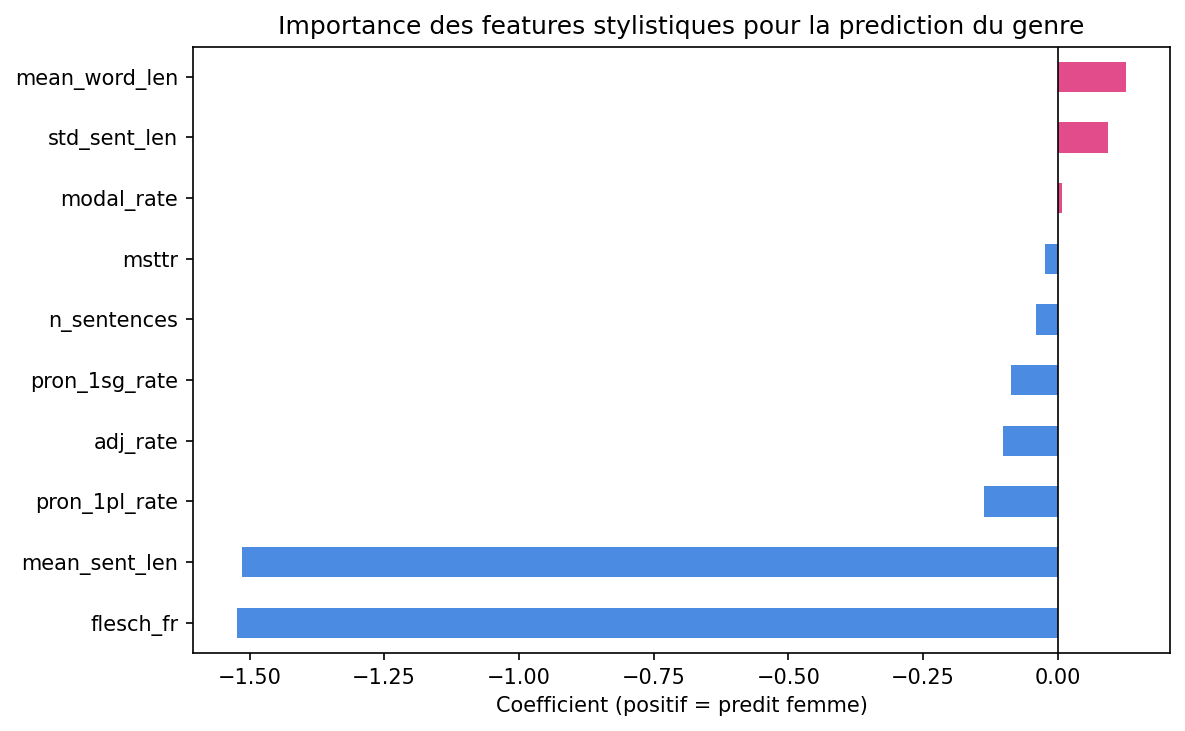
\includegraphics[width=0.70\textwidth]{../figures/04_feature_importance.png}
\caption{Top 20 features par coefficient de régression logistique.
Rose~: features associées au style féminin~; bleu~: features associées
au style masculin. Les valeurs sont les coefficients réels (non absolus).}
\label{fig:feat_imp}
\end{figure}

% ── 5. Discussion ─────────────────────────────────────────────────────────────
\section{Discussion}
\label{sec:discussion}

\subsection{Ce que la modélisation thématique révèle}

La comparaison des trois modèles illustre bien la complémentarité des approches.
La LDA et la NMF sont les outils les mieux adaptés à ce corpus~: en exploitant
les cooccurrences lexicales, elles révèlent des structures thématiques qui
correspondent directement aux clivages politiques historiquement documentés
de 1993. La qualité des thèmes LDA ($C_v = 0.654$) est satisfaisante pour un
corpus politique, un domaine où le vocabulaire partagé est intrinsèquement
élevé.

Le résultat le plus frappant de la section de topic modeling est peut-être
la distinction automatique du Parti de la Loi Naturelle. Ce mouvement avait
la particularité de présenter des candidats dans chaque circonscription avec
un texte quasi identique~--- le modèle l'isole comme un thème à part entière,
ce qui illustre à la fois la puissance et les limites de la LDA~: elle est
très sensible aux patterns lexicaux répétitifs, quelle qu'en soit la nature.

BERTopic échoue à segmenter le corpus pour une raison structurelle~: les
professions de foi sont toutes du même genre discursif, avec le même registre
formel et le même cadre thématique général. Dans l'espace des embeddings, cette
homogénéité de surface efface les différences politiques que les approches
sac-de-mots détectent aisément. Ce résultat suggère que BERTopic est plus
approprié pour des corpus où les documents appartiennent à des genres ou des
domaines très différents.

\subsection{Ce que l'analyse stylistique révèle~--- et ce qu'elle ne révèle pas}

Le signal de genre identifié dans ce corpus est réel mais modeste.
Il réside dans la \emph{structure syntaxique} plutôt que dans le vocabulaire.
Les femmes candidates construisent des phrases avec des groupes nominaux plus
développés (déterminants, nominalisations), une coordination plus explicite,
et un recours plus fréquent aux marqueurs d'atténuation.
Les hommes se distinguent par un ancrage référentiel plus fort dans les noms
propres (personnalités, lieux, institutions).

Ces patterns correspondent à ce que la littérature appelle parfois la
distinction entre style «~implicatif~» (centré sur les relations, les processus,
les nuances) et style «~référentiel~» (centré sur les entités et les faits
\citep{argamon2003gender, lakoff1975language}). Toutefois, deux mises en garde
s'imposent.

Premièrement, les tailles d'effet sont faibles ($r \approx 0.05$--$0.07$),
ce qui signifie que la variabilité intra-groupe est bien plus grande que la
variabilité inter-genre. Il serait abusif de conclure qu'hommes et femmes
«~écrivent différemment~»~: les différences observées sont des tendances
statistiques agrégées sur des milliers de documents, pas des marqueurs individuels.

Deuxièmement, l'absence d'effet pronominal (le «~je~» et le «~nous~» ne sont
pas significatifs après contrôle du parti) est instructive~: les différences
de positionnement énonciatif entre hommes et femmes disparaissent une fois
les partis contrôlés. Cela suggère que c'est davantage la culture partisane~---
le style Lutte Ouvrière vs. le style Verts~--- que le genre qui structure
l'énonciation.

\subsection{Limites et perspectives}

Plusieurs limites méritent d'être explicitées.
La qualité des transcriptions OCR varie selon l'état des documents originaux~:
malgré le pipeline de correction, certains textes présentent encore du bruit
lexical, notamment pour les documents les plus anciens ou de moindre résolution.
Le déséquilibre de genre (88\,\%/12\,\%) réduit la puissance des tests
statistiques pour les features à forte variance et crée un problème de
classification inhérent.
L'analyse est limitée à une seule élection~: la généralisation à d'autres
cycles électoraux ou à d'autres pays francophones resterait à établir.

La principale perspective serait de conduire une analyse longitudinale sur
l'ensemble du corpus Archelec (1958--2022), ce qui permettrait d'étudier
l'évolution du style partisan et du signal de genre au fil des décennies,
et de mesurer l'effet de la loi sur la parité (2000) sur les pratiques discursives.

% ── 6. Conclusion ─────────────────────────────────────────────────────────────
\section{Conclusion}
\label{sec:conclusion}

Ce travail a soumis 5\,835 professions de foi des législatives françaises de
1993 à une analyse computationnelle en deux volets.

Sur le plan thématique, la LDA avec $K=10$ produit des thèmes politiquement
cohérents et interprétables qui reflètent fidèlement la géographie idéologique
de 1993. La spécialisation des partis est forte et asymétrique~: les formations
de niche (FN, extrême gauche, CPNT) sont thématiquement concentrées, tandis
que les partis de gouvernement présentent un discours plus généraliste.
La NMF confirme ces structures avec des thèmes plus contrastés.
BERTopic révèle les limites de l'approche par embeddings sur un corpus homogène
en genre discursif.

Sur le plan stylistique, neuf features sont robustes aux deux protocoles de
test~: les femmes candidates écrivent avec une structure nominale plus développée,
plus coordonnée et plus atténuée~; les hommes avec une densité de noms propres
référentiels plus élevée. Ces différences sont significatives mais d'ampleur
modeste, et elles ne permettent pas une classification individuelle fiable.
Le signal de genre dans les professions de foi est avant tout syntaxique,
non lexical, et distinct du signal partisan.

Ces résultats ouvrent plusieurs pistes~: l'extension longitudinale sur l'ensemble
du corpus Archelec, l'application à d'autres types de discours politiques
formels (programmes de partis, discours parlementaires), et le recours à des
modèles de langue fine-tunés pour mesurer des dimensions stylistiques plus
fines que celles accessibles via les features à base de règles.

% ── Bibliographie ─────────────────────────────────────────────────────────────
\bibliographystyle{abbrvnat}
\bibliography{references}

\end{document}
